\documentclass[11pt,a4paper]{ctexart}
\usepackage[margin=2cm]{geometry}
\usepackage{amsmath,amssymb,bm}
\usepackage{booktabs,graphicx,xcolor,hyperref}
\hypersetup{colorlinks=true,linkcolor=blue,urlcolor=blue}
\setlength{\parindent}{2em}
\setlength{\parskip}{0.25em}
\title{IMU--UWB InEKF：右不变协方差与门限一致性修复}
\author{原论文/代码归因、公式修复与完整数据验证}
\date{2026年7月23日}

\begin{document}
\maketitle

\section{错误归因}

公开提交 \texttt{f3b664e} 已经存在两个实现问题，并非后续改进引入。
原代码先用左坐标雅可比与右不变协方差做门限，
\begin{equation}
 S_{\mathrm{wrong}}=H_lP_rH_l^{\mathsf T}+R,
\end{equation}
随后才执行 $H_r=H_l\operatorname{Ad}_{\hat X^{-1}}$。此外，带有普通姿态、速度、
位置标准差含义的对角 $P_0$ 被直接作为右不变误差协方差，没有坐标映射。

论文式 (17) 定义 $\eta^r=\hat X X^{-1}$。由
\begin{equation}
 \xi^l=\operatorname{Ad}_{X^{-1}}\xi^r
\end{equation}
得到 $H_r=H_l\operatorname{Ad}_{\hat X^{-1}}$。论文式 (38) 印为
$H_r=H_l\operatorname{Ad}_{\hat X}$，与该关系及公开代码不一致，至少存在记号或漏写
逆矩阵的疑点。本次没有把代码机械改成式 (38) 的字面形式。

\section{协方差与门限修复}

若 $P_l$ 表达普通物理/局部先验，则右不变协方差应初始化为
\begin{equation}
 \boxed{
 P_r=\operatorname{Ad}_{\hat X}P_l\operatorname{Ad}_{\hat X}^{\mathsf T}}
 \label{eq:cov-map}
\end{equation}
并在雅可比转换后只计算一次门限：
\begin{align}
 H_r&=H_l\operatorname{Ad}_{\hat X^{-1}},\\
 S&=H_rP_rH_r^{\mathsf T}+R,\\
 \mathrm{NIS}&=z^2/S,\qquad
 \mathrm{reject}\Longleftrightarrow\mathrm{NIS}\ge25.
\end{align}
由式~\eqref{eq:cov-map}，
\begin{equation}
 H_rP_rH_r^{\mathsf T}
 =H_lP_lH_l^{\mathsf T},
\end{equation}
因此共同平移机体和全部基站不会改变创新统计量。

\section{全圆未知航向先验}

论文采用 $\sigma_\psi=1$ rad，却测试 $\pi$ rad 初差；后者是 3.14$\sigma$ 事件。
对全圆未知航向，均匀分布的等效标准差为
\begin{equation}
 \sigma_{\mathrm{uniform}}
 =\sqrt{\frac{1}{2\pi}\int_{-\pi}^{\pi}\psi^2\,d\psi}
 =\frac{\pi}{\sqrt3}\approx1.814~\mathrm{rad}.
\end{equation}
修复版采用保守的 $\sigma_\psi=2.0$ rad。它不读取真实初差，只表达全圆未知先验。

\section{30秒全角度结果}

六条 manual 轨迹分别测试 $0^\circ,90^\circ,120^\circ,150^\circ,180^\circ$。
修复前 const3 大角度位置 RMSE 为 36.8--560.8 m；修复后全部 30 个条件为
0.208--0.431 m，UWB 拒绝率为 0.249\%--2.17\%。

\begin{figure}[htbp]
\centering
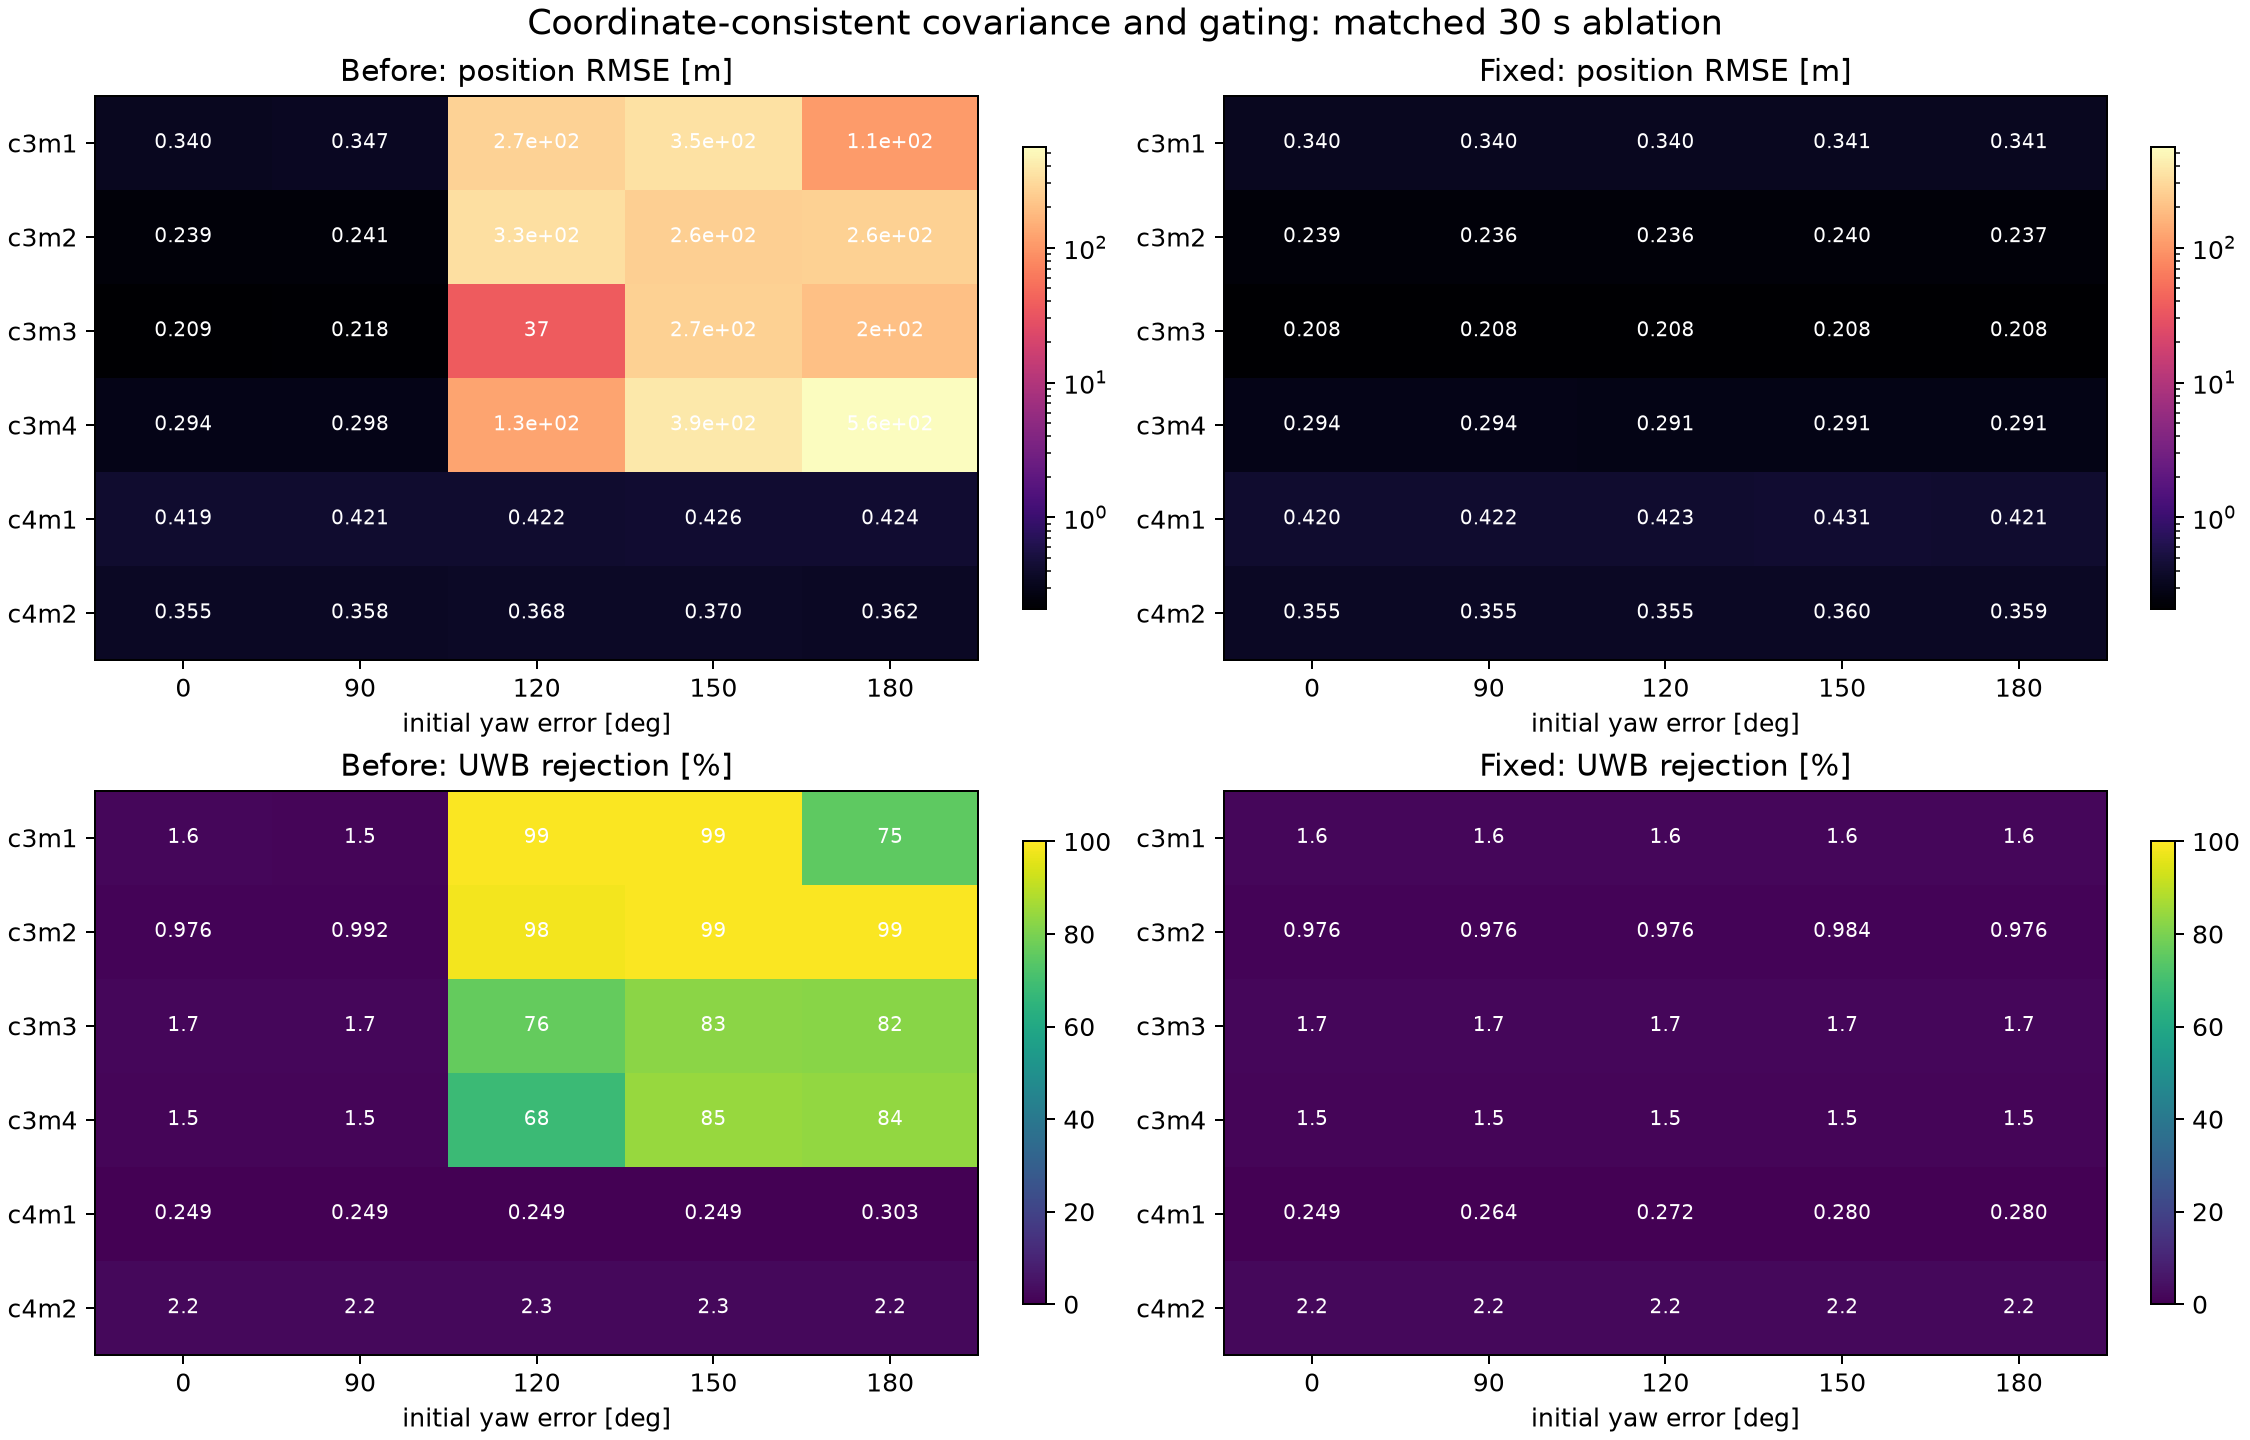
\includegraphics[width=\textwidth]{../imu-uwb-inekf/results/coordinate_fix_final/01_grid_metrics.png}
\caption{30 s 配对网格。修复后没有大角度门限锁死。}
\end{figure}

\section{完整60秒、180度初差}

\begin{table}[htbp]
\centering
\caption{完整 60 s before/after 配对结果}
\begin{tabular}{lrrrrr}
\toprule
数据 & 位置前/m & 位置后/m & yaw前/rad & yaw后/rad & 拒绝率前/后\\
\midrule
c3m1 & 1983.350 & 0.283 & 1.644 & 0.112 & 74.39\%/1.19\%\\
c3m2 & 1350.634 & 0.275 & 2.740 & 0.180 & 99.62\%/1.42\%\\
c3m3 & 571.757  & 0.206 & 2.657 & 0.226 & 83.34\%/1.58\%\\
c3m4 & 2386.810 & 0.288 & 3.093 & 0.138 & 85.69\%/1.72\%\\
c4m1 & 0.357 & 0.355 & 0.123 & 0.131 & 0.60\%/0.59\%\\
c4m2 & 0.337 & 0.335 & 0.172 & 0.114 & 1.52\%/1.50\%\\
\bottomrule
\end{tabular}
\end{table}

\begin{figure}[htbp]
\centering
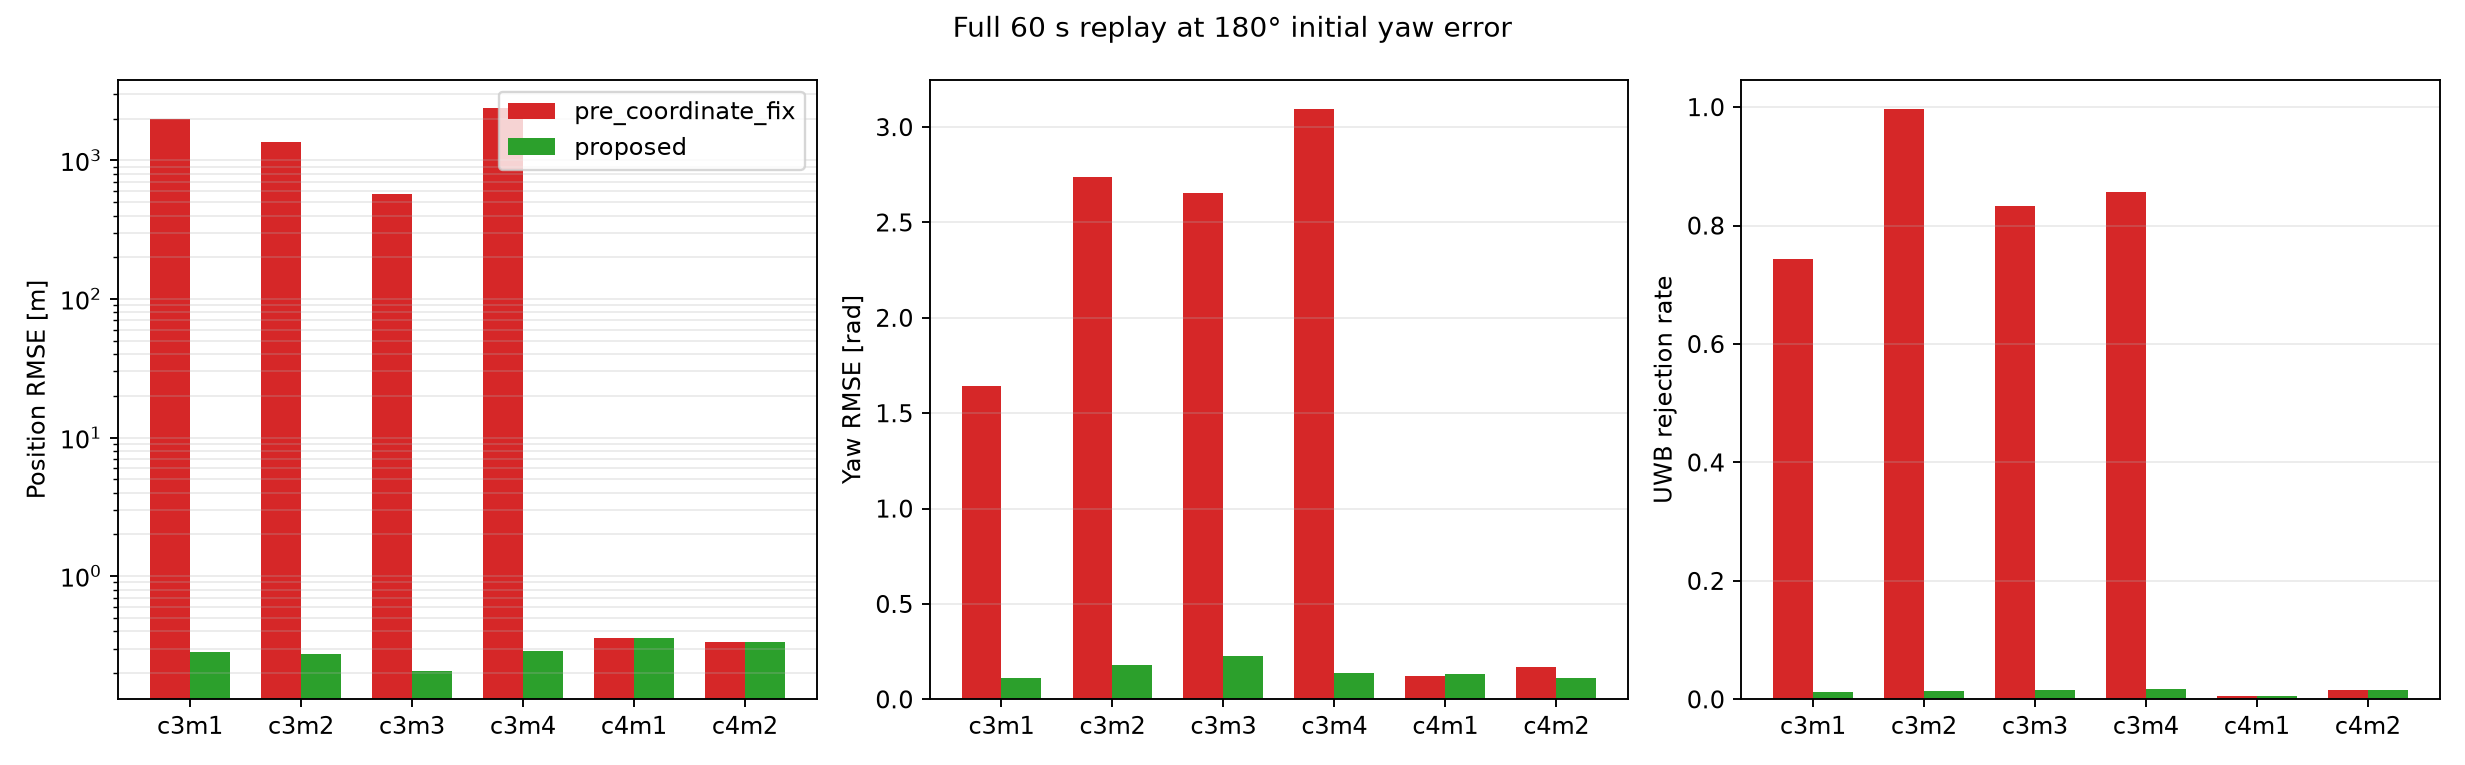
\includegraphics[width=\textwidth]{../imu-uwb-inekf/results/coordinate_fix_full60/full60_before_after.png}
\caption{完整 60 s、180$^\circ$ 初差。const3 从发散恢复，同时保持 const4。}
\end{figure}

\section{坐标平移反事实}

物理轨迹与基站共同平移后，修复前 const3-manual3 的位置 RMSE 可由
197.474 m 变成 0.211 m，const4-manual1 可由 0.424 m 变成 369.055 m。
修复后两种原点的结果分别严格一致为 0.208252 m 和 0.421342 m。

\begin{figure}[htbp]
\centering
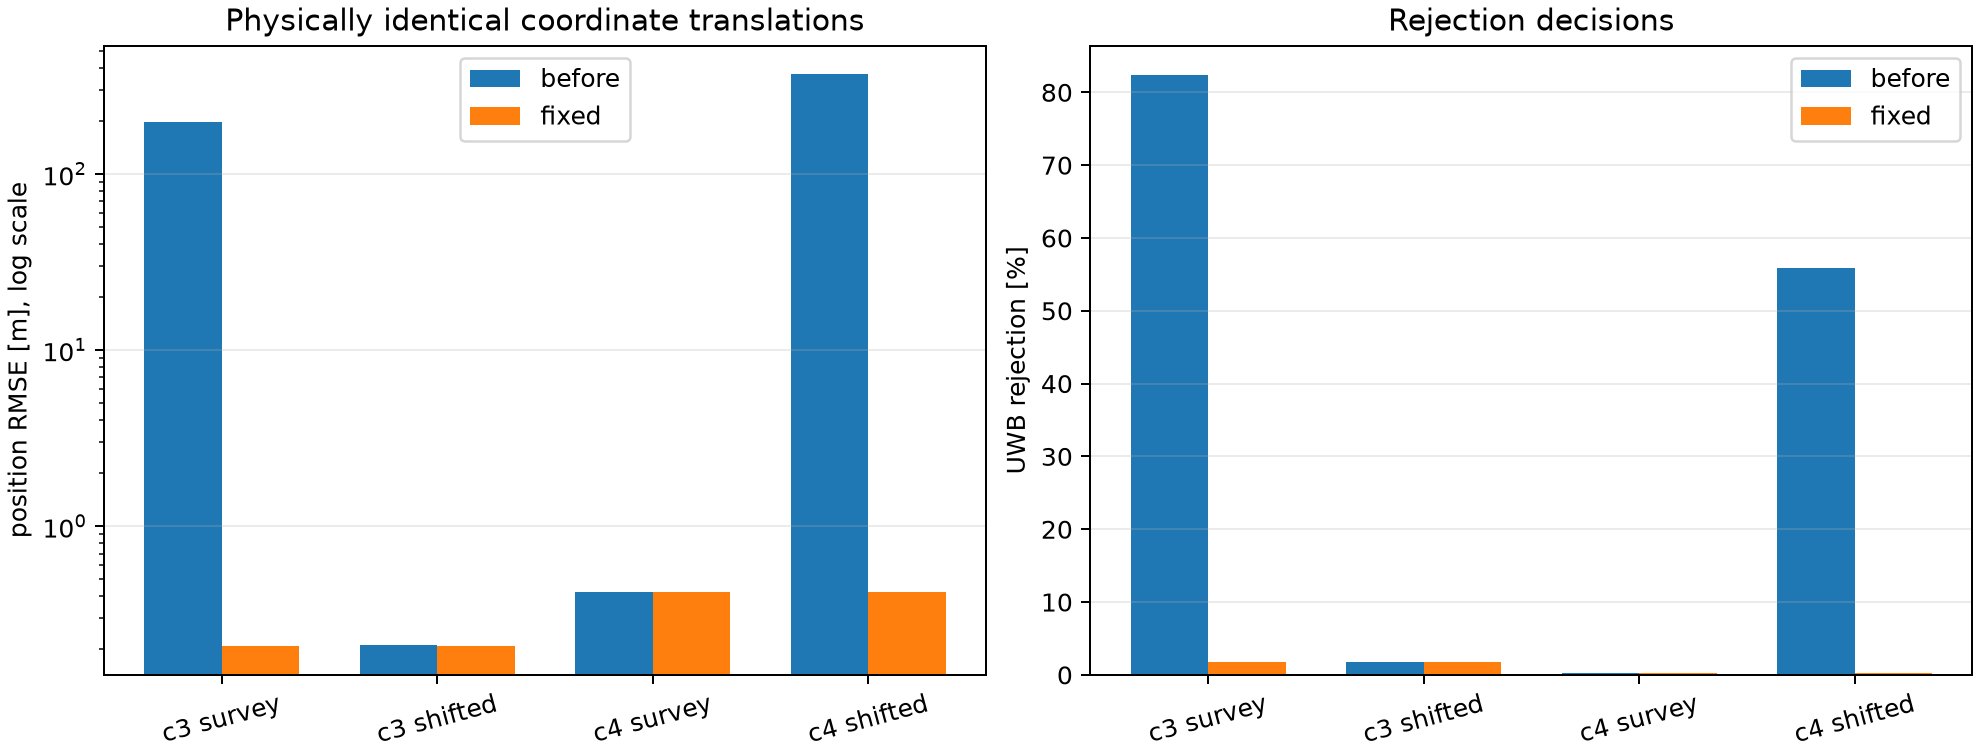
\includegraphics[width=\textwidth]{../imu-uwb-inekf/results/coordinate_fix_final/02_translation_invariance.png}
\caption{修复消除了世界坐标原点对物理结果的影响。}
\end{figure}

\section{限制与计算量}

修复只在初始化增加一次 $15\times15$ 协方差映射，并删除每个 UWB 样本的一次重复
预门限，滤波循环渐近复杂度不增加。c3m3 修复后 yaw RMSE 为 0.226 rad（约
13$^\circ$），已恢复可用但仍非高精度航向；若要求长期小于 5$^\circ$，仍需额外
可观测信息或更系统的圆周先验，而不能通过改变评价区间美化。

\end{document}
